\label{sec:websiteimplementation}
The website is built to allow exhibition organisers to manage their exhibition, as stated in the problem statement \secref{sec:problemstatement}. All concepts of an exhibition can be added from the website, this include feeds, schedule, booths, companies, categories and a floor plan. The website is split up into different tabs. The different tabs manage different concepts of an exhibition:

\begin{description}
	\item[Feeds] In the "Feeds" tab the organiser can add a feed to a booth in the database.
	\item[Company] In the "Company" tab the organiser can add a company to the database, the company logo will also be uploaded to the server for further use.
	\item[Category] In the "Category" tab the organiser can add a category to the database for further use.
	\item[Exhib] In the "Exhib" tab the organiser can create a new empty exhibition.
	\item[Schedule] In the "Schedule" tab the organiser can create a new schedule and add it to a booth in the database.
	\item[Floor plan] The "Floor plan" tab is the heart of the website, here almost all the other concepts can be added, this include making a new exhibition complete with a floor plan, categories, companies, and booths. Previous created exhibitions can also be loaded for viewing or editing.
\end{description}

The problem statement \secref{sec:problemstatement} states that booths should be able to create feeds themselves, this has not been used in the design of the website, but it is possible with the integration of a login system on the website. This will also make sure only the organisers will be able to edit their own exhibitions.

The website is designed with the main focus on the "Floor plan" tab, this tab functions almost as a standalone one-page website, though the "Feed" and "Schedule" tab is also needed to make a "complete" exhibition.

The "Floor plan" tab makes use of the Google Maps \ac{api}, giving a visual presentation when creating an exhibition.
The following steps are required when creating an exhibition floor plan:
\begin{description}
	\item[Step 1] Click the "Create Exhibition" button and fill in the exhibition information.
	\begin{figure}[H]
		\centering
		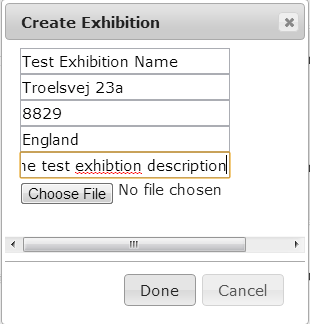
\includegraphics[scale=0.5]{img/website/step2.png}
		\caption{Create exhibition dialogue.\label{fig:websitestep1}}
	\end{figure}
	\item[Step 2] Create a number of markers, which will make up the walking path of the exhibition floor.
	\begin{figure}[H]
		\centering
		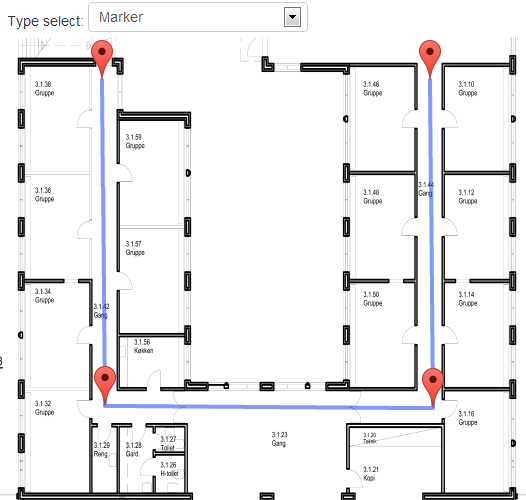
\includegraphics[scale=0.5]{img/website/step3.png}
		\caption{Floor plan walking path.\label{fig:websitestep2}}
	\end{figure}
	\item[Step 3] Create a booth by having selected the "Booth" option, and clicking the floor plan in any given position. When the booth positioning and size is correct, the booth can be locked by clicking it again, this will bring up the "Booth information" dialogue. Fill in the booth information, and the booth will be saved.
	\begin{figure}[H]
		\centering
		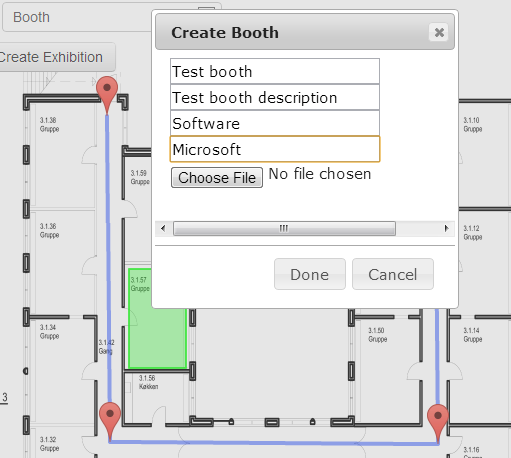
\includegraphics[scale=0.5]{img/website/step4.png}
		\caption{Create booth dialogue.\label{fig:websitestep3}}
	\end{figure}
	\item[Step 4] Repeat step 3, until all booths have been created.
	\item[Step 5] Bind the locked booths by right-clicking them, and then clicking a point on the walking path. This will create a new entry point for the booth.
	\begin{figure}[H]
		\centering
		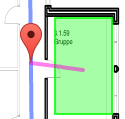
\includegraphics[scale=0.5]{img/website/step5.png}
		\caption{Booth entry point on walking path.\label{fig:websitestep5}}
	\end{figure}
	\item[Step 6] Repeat step 5 until all booths are bound to the walking path, a booth can have multiple entry points.
	\item[Step 7] Save the exhibition by clicking the "Save" button. This will save the exhibition to the database.
\end{description}
For a better overview of creating an floor plan using this feature see \autoref{fig:floorplan}.

\begin{figure}[H]
	\centering
	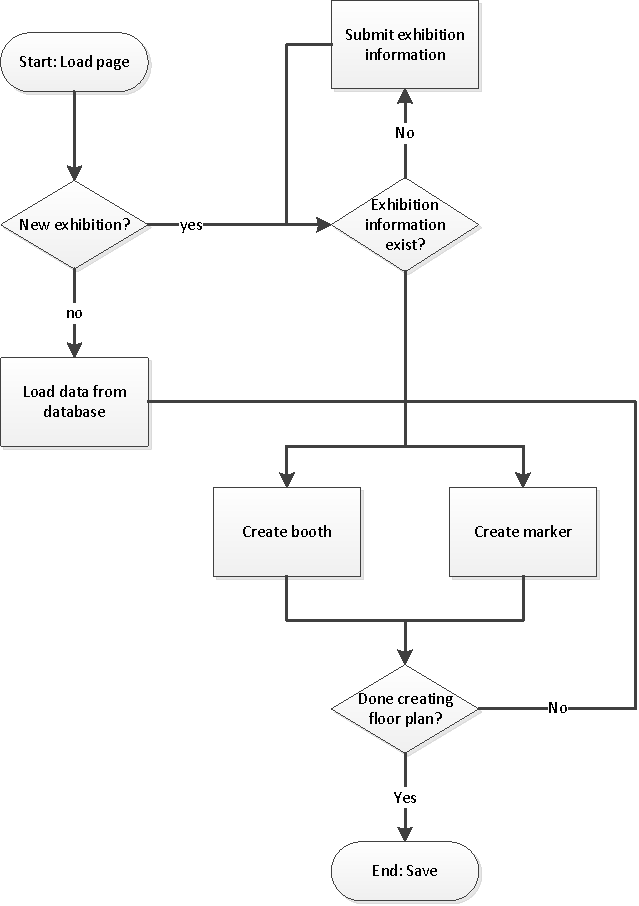
\includegraphics[width=0.7\linewidth]{img/floorplanflow.pdf}
	\caption{Flowchart of creating a floor plan.\label{fig:floorplan}}
\end{figure}

After creating an exhibition the organiser can add feeds to the exhibition, using the "Feeds" tab, feeds are bound to an existing booth from the database. A schedule can be added using the "Schedule" tab, here the organiser selects a "Name", "Booth", "Start time" and "End time".
It is also possible to load an existing exhibition from the database, for the loaded exhibition the floor plan will be shown on the map. This exhibition can then be edited, and the changes can be saved to the database.

All form requests on the website are handled using the AJAX technology\citep{ajax}. AJAX is a technique allowing a website to be dynamically updated while the user is looking at it. The AJAX scripts post form data to PHP, which handles the database interaction. When connecting to the database prepare statements are used, to make sure no malicious data is inserted into the database.

An important missing feature on the website is the limitation of the custom tile set when making a floor plan. For the time being it is a fixed set of tiles.

The design of the website is done using Twitter Bootstrap\citep{twitterbootstrap}, a CSS \ac{ui} supplying a stylish and uniform interface.
Our main focus on the website was functionality and therefore the graphic design and usability was not the main priority.
